\documentclass[]{report}   % list options between brackets
\usepackage{}              % list packages between braces
\usepackage[spanish]{babel}
\usepackage{electComp}
\usetikzlibrary{decorations,decorations.pathmorphing,decorations.pathreplacing}
\usepackage{tikz}
\usepackage{url}


% type user-defined commands here

\begin{document}

\title{Proyecto 1: Fuente de poder}   % type title between braces
\author{Carlos L\'{o}pez (08107) y Josu\'{e} Rend\'{o}n (08168)}         % type author(s) between braces
\date{7 de Mayo, 2010}    % type date between braces
\maketitle

\begin{abstract}
Constru\'{i}mos una fuente de alimentaci\'{o}n que toma como entrada 110V y tiene como salida un voltaje variable que va desde 1V hasta 20V. El tipo de fuente que constru\'{i}mos es una fuente de voltaje lineal, es decir, que est\'{a} compuesta por 4 m\'{o}dulos esenciales y uno de seguridad. Estos m\'{o}dulos son: 

\begin{enumerate}
\item M\'{o}dulo de reductor de voltaje
\item M\'{o}dulo de rectificaci\'{o}n
\item M\'{o}dulo de filtrado
\item M\'{o}dulo de regulaci\'{o}n
\end{enumerate}

El m\'{o}dulo de seguridad consiste en tres fusibles que evita que al alimentar nuestra fuente con un voltaje mayor al necesario se da\~{n}e y que al momento que nuestra fuente proporcione m\'{a}s voltaje del especificado, queme los instrumentos que est\'{a}n conectados a la misma. El tiempo que tom\'{o} constru\'{i}rla fue de aproxim\'{a}damente 8 horas, sin tomar el cuenta del tiempo de comprar los materiales, tubo un costo de aproxim\'{a}damente 150 quetzales guatemaltecos.

\end{abstract}

\chapter{Introducci\'{o}n}           % chapter 1
%\section{History}       % subsection 1.1.1
Una fuente de poder se conoce como el m\'{o}dulo encargado de energizar adecuadamente un dispositivo electr�nico. En el caso espec\'{i}fico de circuitos el\'{e}ctricos, interesa alimentar circuitos de relativamente baja potencia con corriente continua, es decir, invariante en el tiempo. 

Existen b\'{a}sicamente dos formas de alimentar correctamente un circuito electr�nico: 
\begin{enumerate}
\item Pilas o bater\'{i}as
\item Un circuito que convierta corriente alterna (desde un toma-corriente 110V) a corriente directa.
\end{enumerate}

\'{E}ste trabajo consta de varias fases o etapas que describen la construcci\'{o}n de la segunda, de una fuente de voltaje lineal.

\chapter{Dise\~{n}o esperimental}     

La fuente dise\~{n}ada es una fuente l\'{i}neal, es decir que, sigue el esquema: reductor de voltaje, rectificador, filtrado, regulaci\'{o}n y salida. En resumen, el reductor de voltaje adapta el valor de tensi\'{o}n o voltaje de entrada. Luego, el rectificador convierte ese voltaje AC en DC para que el filtrado disminuya el rizado de la componente alterna con un condensador o capacitor. Finalmente se regula el valor de la tensi\'{o}n de salida.

\section{Transformador reductor de voltaje}  
\subsection{Materiales utilizado}
\begin{center}\begin{tabular}{ r | l } \textbf{Cantidad} & \textbf{Descripci\'{o}n} \\ \hline 1 & Transformador con Tab-central de 110V a 15+15V de 1ra. \end{tabular}
\end{center}

\subsection{Descripci\'{o}n}
El objetivo de esta etapa, la primer etapa, es el de convertir un voltaje de 110Vrms A.C. comunmente encontrado en un toma-corriente cualquiera en un voltaje que se pueda utilizar en un circuito el\'{e}ctrico, generalmente los voltajes son m\'{a}s bajos para estos por lo que esta etapa consiste en reducir el voltaje de 110V a 12V tambi\'{e}n en corriente alterna.

\subsection{Implementaci\'{o}n}

\section{Rectificador}
\subsection{Materiales utilizado}
\begin{center}\begin{tabular}{ r | l } \textbf{Cantidad} & \textbf{Descripci\'{o}n} \\ \hline 4 & Diodos 1N4001 \end{tabular}
\end{center}

\subsection{Descripci\'{o}n}
El objetivo de esta etapa es la de convertir el voltaje de salida del transformador de 12V de corriente alterna en 12V de corriente directa, es decir eliminar el componente negativo de la se\'{n}al de salida del transformador.

\subsection{Implementaci\'{o}n}
Se utilizaron 4 diodos configurados de la manera mostrada en la Figura \#2
\begin{center}
\begin{tikzpicture}[line width=1pt] 
   \coordinate (enmedio) at (8:0cm);
    \draw (0,2cm) -- ++(2cm,0cm);
    \draw (0,0cm) -- ++(2cm,0cm);
    \draw (1,1) -| ++ (-0.5,1.2); 
    \draw (0.5,2.2) -- ++ (3.5,0);
    \draw (3,1) -- ++ (1,0);    
    \draw[decorate, decoration=diode] (1cm,1cm) -- ++ (1cm,1cm) ; 
    \draw[decorate, decoration=diode] (2cm,2cm) -- ++ (1cm,-1cm);
    \draw[decorate, decoration=diode] (1cm,1cm) -- ++ (1cm,-1cm);
    \draw[decorate, decoration=diode] (2cm,0cm) -- ++ (1cm,1cm);
    \node (vt) at (-0.25,1) {$V_{t}$};
    \node [above of=vt] {+};
    \node [below of=vt] {$-$};
    \node (vf) at (4.2,1.6) {$V_r$};
    \node at (4.2,2.2cm) {$-$};
    \node at (4.2,1) {+};
\end{tikzpicture}\\
Figura \#2
\end{center}

\section{Filtrado}
\subsection{Materiales utilizado}
\begin{center}\begin{tabular}{ r | l } \textbf{Cantidad} & \textbf{Descripci\'{o}n} \\ \hline 2 & Capacitores de 1000$\mu$F/25V
\end{tabular}
\end{center}

\subsection{Descripci\'{o}n}
Esta etapa tiene como objetivo convertir el voltaje que sale de la etapa de filtrado $V_r$ que es corriente directa, en m\'{a}s 'constante', es decir, que var\'{i}e lo menos posible respecto al tiempo. Este resultado se obtiene cuando el capacitor da la energ\'{i}a acomulada necesaria cuando la se\'{n}al de salida disminuye hacia cero.

\subsection{Implementaci\'{o}n}
Se usaron dos capacitores,  configurados como se muestra en la Figura \#3

\begin{center}
\begin{tikzpicture}[line width=1pt] 
\def\ground{%
    -- +(0mm,-4.0mm) {
        [yshift=-4mm]
        +(-2mm,0mm) -- +(2mm,0mm)
                +(-1mm,-1mm) -- +(1mm,-1mm)
                +(-0.3mm,-2mm) -- +(0.3mm,-2mm)
        }
}

   \draw (0,0) -- ++ (3,0);
   \draw (0,2) -- ++ (3,0);
   \draw[decorate,decoration=capacitor] (1,0) -- ++ (0,1);
   \draw[decorate,decoration=capacitor] (1,1) -- ++ (0,1);
   \draw (3,1) \ground;
   \draw (1,1) -- ++ (2,0);
    \node (vt) at (-0.25,1) {$V_{r}$};
    \node [above of=vt] {+};
    \node [below of=vt] {$-$};
    \node (vf) at (4.2,1) {$V_f$};
    \node at (4.2,2cm) {$+$};
    \node at (4.2,0) {$-$};
\end{tikzpicture}\\
Figura \#3
\end{center}

\section{Regulaci\'{o}n de voltaje} 
\subsection{Materiales utilizado}
\begin{center}\begin{tabular}{ r | l } \textbf{Cantidad} & \textbf{Descripci\'{o}n} \\ \hline 
1 & Integrado LM317T con disipador de calor\\
1 & Integrado LM337 con disipador de calor \\
2 & Potenciometros 5kOhms \\
2 & Resistencias de 220 Ohms  \end{tabular}
\end{center}

\subsection{Descripci\'{o}n}
Con la ayuda de una resistencia variable y una de 220 Ohms para cada se\~{n}al, los circuitos integrados son capaces de proveer el voltaje de salida requerido. Estos circuitos son los principales encargados de regular el voltaje de salida de la fuente.

\subsection{Implementaci\'{o}n}
Los dos circuitos integrados (uno para se\~{n}al negativa y otra para positiva) cada uno junto con las dos resistencias (una de 220 y la otra variable) se configuraron acorde a la Figura \#4.
\begin{center}
\begin{tikzpicture}[line width=1pt] 
\def\ground{%
    -- +(0mm,-4.0mm) {
        [yshift=-4mm]
        +(-2mm,0mm) -- +(2mm,0mm)
                +(-1mm,-1mm) -- +(1mm,-1mm)
                +(-0.3mm,-2mm) -- +(0.3mm,-2mm)
        }
}

   \draw (0,0) -- ++ (2,0);
   \draw (0,4) -- ++ (2,0);
   
   \draw (3,0) -- ++ (3,0);
   \draw (3,4) -- ++ (3,0);
   
   \draw (2.5,0.5) -- ++ (0,0.5);
   \draw (2.5,3.5) -- ++ (0,-0.5);	
   
   \draw (2.5,1) -- ++ (2,0);
   \draw (2.5,3) -- ++ (2,0);
   
   \draw (3.5,2) -- ++ (2,0);
   \draw (5.5,2) \ground;
   
   \draw [decorate,decoration=resistor] (3.5,1) -- ++ (0,1);
   \draw [decorate,decoration=resistor] (3.5,2) -- ++ (0,1);
   
   \draw [decorate,decoration=resistor] (4.5,0) -- ++ (0,1);
   \draw [decorate,decoration=resistor] (4.5,3) -- ++ (0,1);
   
   \draw [decorate,decoration=resistor] (4.5,0) -- ++ (0,1);
   
   %cajitas
   \draw (2,0) |- ++ (1,0.5);
   \draw (3,0.5) |- ++ (-1,-1);
   \draw (2,-0.5) -- ++ (0,0.5);
   
   \draw (2,4) |- ++ (1,0.5);
   \draw (3,4.5) |- ++ (-1,-1);
   \draw (2,3.5) -- ++ (0,0.5);
   %\draw 
    \node (vt) at (0,2) {$V_{f}$};
    \node [above of=vt] {+};
    \node [below of=vt] {$-$};
    \node (vout) at (6.5,2) {$V_{out}$};
    \node [above of=vout] {$+$};
    \node [below of=vout] {$-$};
    
    \node (lm1) at (2.5,0) {\tiny LM337};
    \node (lm2) at (2.5,4) {\tiny LM317T};
    
    \node (lm1) at (5.45,0.5) {\tiny 220 Ohms};
    \node (lm1) at (5.45,3.5) {\tiny 220 Ohms};
\end{tikzpicture}\\
Figura \#4
\end{center}

\section{Seguridad}
\subsection{Materiales utilizado}
\begin{center}\begin{tabular}{ r | l } \textbf{Cantidad} & \textbf{Descripci\'{o}n} \\ \hline 3 & Fusibles de 1A \\ 2 & Resistencias de 1k Ohms \end{tabular}
\end{center}

\subsection{Descripci\'{o}n}
Esta secci\'{o}n de la fuente de alimentaci\'{o}n es opcional, pero de vital importancia si no queremos que los circuitos alimentados con nuestra fuente sufran da\'{n}os.

\subsection{Implementaci\'{o}n}
Se coloc\'{o} un fusible en cada salida (positiva y negativa) junto con una resistencia de 1k Ohm y antes del transformador.

\chapter{Resultado y Discusi\'{o}n}
El proyecto tubo como resultante una fuente de voltaje en donde se demostr\'{o} el correcto funcionamiento de la misma: Se hizo una muestra de aproximadamente 5 intentos en el que el voltaje de salida resultante variaba desde 1V hasta 20V en corriente directa, es decir se encontraba en el rango de (1V,20V).

La fuente de alimentaci\'{o}n constru\'{i}da funciona si y solo si los 4 primeros m\'{o}dulos o etapas funcionan (Reductor de voltaje, rectificador, filtrado y regulaci\'{o}n), cada uno es de vital importancia y aqu\'{i} se discutir\'{a} que aporta cada uno y que rol juega en la construcci\'{o}n.

\section{Reductor de voltaje}
El transformador es un dispositivo que se encarga de "transformar" el voltaje de corriente alterna que tiene en su entrada, a otro voltaje con diferente amplitud, ,que entrega en su salida. Est\'{a} compuesto de un n\'{u}cleo de hierro sobre el cual se encuentran enrolladas varias vueltas de un alambre conductor (dos bobinas). La primera bobina, $B_1$, es que recibe el voltaje de entrada $V_o$ y la segunda,$B_2$,la que entrega el voltaje transformado $V_s$.

La bobina $B_1$ recibe un voltaje $V_o$ alterno que circular\'{a} por ella una corriente alterna, \'{e}sta induce un flujo magn\'{e}tico en el n\'{u}cleo de hierro. Al haber un flujo magn\'{e}tico que atraviesa la bobina $B_2$, se generar\'{a} por el alambre un voltaje $V_s$. 

La raz\'{o}n de transformaci\'{o}n del voltaje entre $B_1$ y $B_2$ depende del n\'{u}mero de vueltas que tenga cada una. Si el n\'{u}mero de vueltas de $B_2$ es el triple de $B_1$, $V_s$ ser\'{a} tres veces $V_o$. 

Por lo tanto, 

\begin{equation}
V_s = N_s * \frac{V_o}{N_o}
\end{equation}
 
En donde $N_s$ y $N_o$ representan el n\'{u}mero de vueltas que da el alambre en $B_2$ y $B_1$ respectivamente.

Un transformador puede elevar o reducir el voltaje, en nuestro caso, lo reducimos a 12V. La amplitud de $V_s$ es de vital importancia para el circuito, en este caso de 12V. Saber esta amplitud nos permite saber con que voltaje m\'{a}ximo se est\'{a} trabajando y por ejeplo en el m\'{o}dulo de filtrado, que valores de capacitancia necesitamos para mantener el valor de voltaje constante. 

\section{Rectificador}
El m\'{o}dulo de rectificaci\'{o}n consiste en 4 diodos. Cada diodo permite que pase la corriente en solo una direcci\'{o}n, en la Figura \# 3 se muestra una configuraci\'{o}n de 4 diosos, llamado Puente de diodos. El puente de diodos recibe un voltaje con corriente alterna, es decir, positivo o negativo con una amplitud de 12V. Los dos diodos de arriba conducen la tensi\'{o}n (voltaje) positiva y cuando la tensi\'{o}n de la se\'~{n}al es negativa, los dos diodos de abajo conducen la tensi\'{o}n negativa.

Esto permite que la se\~{n}al de corriente alterna, se convierta en corriente directa, es decir positiva, como se muestra a continuaci\'{o}n en la Figura \#6.

\begin{center}
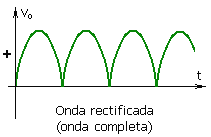
\includegraphics[scale=0.7]{tension_rectificada.png}\\
Figura \#6
\end{center} 

\section{Filtrado}
La secci\'{o}n de filtrado, tiene como objetivo volver la se\~{n}al m\'{a}s 'constante', esto se logra con un par de condesadores (o capacitores). Un condensador est\'{a} formado por dos placas met\'{a}licas separadas por un material no conductor. Al conectar un condensador a un voltaje, una de las placas se carga e induce una carga de signo opuesto en la otra placa.

Cuando el voltaje de entrada $V_o$ alcanza el m\'{a}ximo de tensi\'{o}n $V_M$, el condensador ha completado su carga y a partir de entonces la se\~{n}al de entrada comienza a disminu\'{i}r. Al ocurrir esto, el condensador intenta descargarse. 

\section{Regulaci\'{o}n}
En el m\'{o}dulo de regulaci\'{o}n se recibe un voltaje mayor al de salida. El regulador act\'{u}a como un "cortador" de voltaje que no deja pasar si no el voltaje indicado y los voltajes superiores son detenidos.

Se utilizaron los circuitos integrados de LM117 y LM337, que tiene 3 terminales para voltajes positivos o negativos respectivamente, estos son capaces de proveer un m\'{a}ximo de 1.5A desde 1.2V a 37V. Son f\'{a}ciles de usar y requieren solamente dos resistencias externas. Una de esas resistencias, de 220 Ohms, est\'{a} conectada en paralelo con el adjunto del integrado, y este en serie con un potenciometro, que es una resistencia variable conectada a tierra.

\section{Seguridad}
El m\'{o}dulo de seguridad consiste en 3 fusibles. Cada fusible permite el paso de la corriente mientras \'{e}ste no supere un valor establecido. Si el valor de la corriente que pasa es superior a \'{e}ste, el fusible se derrite y no deja pasar la corriente.

Un fusible est\'{a} conectado entre la fuente de alimentaci\'{o}n y el circuito de la fuente de voltaje, para proteger nuestro circuito. Los otros dos fusibles, se usan en cada una de las terminales de salida (positiva y negativa) para proteger a los circuitos que se conecen con nuestra fuente de voltaje.
\chapter{Conclusiones}

\begin{itemize}
\item El rectificador de onda completa permite aprovechar el total de la salida del transformador de voltaje, se aprovecha tanto el positivo como el voltaje negativo.
\item La utilizaci\'{o}n de condensadores con valores de capacitancia altos, permite filtrar la se�al rectificada de mejor forma ya que estos pueden almacenar m\'{a}s enegr\'{i}a, los de 1000$\mu$F fueron suficientes.
\item Fue muy importante y clave probar los capacitores antes de soldarlos debido a que en varias ocaciones fallaron, por estar mal conectados. 
\item El transformador de voltaje redujo la tensi\'{o}n pero aument\'{o} el valor de la corriente que entraba, por lo que fue necesario integrar fusibles de 1A.
\item Utilizar cloruro f�rrico calentado caliente redujo considerablemente el tiempo para disolver el cobre.
\end{itemize}

\begin{thebibliography}{9}
Transformador el\'{e}ctrico, Relaci\'{o}n de voltajes, corrientes y potencias en un transformador, Unicrom, \url{http://www.unicrom.com/Tut_transformador.asp} \\ \\
El fusible, Fusible: Protecci\'{o}n contra sobre corrientes y corto circuitos, Unicrom, \url{http://www.unicrom.com/Tut_fusible.asp}\\ \\
Overview, LM317, 3-Terminal Adjustable regulator, National Seiconductor, \url{http://www.national.com/mpf/LM/LM317.html#Overview}.\\ \\
Fuente de alimentaci\'{o}n lineal, Fuente de alimentaci\'{o}n, Wikipedia en espa\~{n}ol, 7 de Mayo 2010, \url{http://es.wikipedia.org/wiki/Fuente_de_alimentaci�n} \\ \\
Fuente de Poder, Diagrama de bloques, Unicrom, \url{http://www.unicrom.com/Tut_fuentepoder.asp} \\ \\
Proceso de descarga de un condensador, Unicrom, \url{http://www.unicrom.com/Tut_descargacondensador.asp} \\ \\
Puente de Graetz o Puende rectificador de doble onda, Rectificador de onda completa, Wikipedia en espa\~{n}ol, \url{http://www.unicrom.com/Tut_descargacondensador.asp} \\ \\
%http://www.unicrom.com/Tut_transformador.asp
  % type bibliography here
\end{thebibliography}

\end{document}